Cette préface est déstinée à tous les lecteurs, toutes les lectrices, et pas
seulement les mathématiciens et mathématiciennes. Après les remerciements
d'usage, on présentera quelques applications des \emph{corps finis}, l'objet au
cœur de ce document, afin de comprendre l'étendue de leur utilité. Celles et ceux
voulant assouvir leur soif de détails techniques et de mathématiques
pourront le faire en parcourant les références bibliographiques proposées. Cela
sera sans doute aussi possible (jusqu'à un certain point) en lisant les autres
chapitres de ce manuscrit, ainsi que la fin de cette préface, qui donne un
résumé détaillé du contenu du document.

\minitoc
% TODO
% ====
%
% Find an illustration (something linked with crypto preferably)
\clearpage

\section*{Remerciements}
\addcontentsline{toc}{section}{Remerciements}

\clearpage
\section*{Applications des corps finis}
\addcontentsline{toc}{section}{Applications des corps finis}

On peut se demander, probablement à juste titre, à quoi sert une thèse en
mathématiques fondamentales. J'ai la chance d'avoir travaillé sur un sujet qui,
quoique relativement abstrait, possède des applications extrêmement utiles, et
ce dans la vie de tous les jours, pour quasiment tout le monde. Nous allons donc
voir deux applications élégantes des \emph{corps finis}, qui illustrent
l'intérêt de ces objets mathématiques.

\subsection*{Cryptography}
\addcontentsline{toc}{subsection}{Cryptographie}
\label{sec:crypto}

Pendant toute la durée de mon doctorat, j'ai expliqué aux non-mathématiciens que
je faisais une thèse en \emph{cryptographie}. C'est en fait un mensonge, car
même si le titre initial du projet de thèse était \emph{Arithmétique efficace
pour la cryptographie et la cryptanalyse}, je me suis finalement intéressé
aux deux premiers mots seulement : arithmétique efficace. Cependant, la
cryptographie reste une source d'inspiration et une des motivations derrière ces
travaux. Les recherches que nous avons menées viennent souvent de la
cryptographie, ou bien ont une application dans cette discipline, nous
commencerons donc par expliquer ce que ``cryptographie'' signifie.

Nous sommes des animaux sociaux, et nous avons donc besoin de communiquer les
uns avec les autres. Parfois, nous voulons que nos échanges restent privés.
Les raisons derrière ce souhait peuvent être multiples : informations
militaires, commerciales, médicales, bancaires, histoires amoureuses... La
cryptographie est la science qui étudie les techniques utilisées pour sécuriser
les communications, en présence d'une tierce partie appelée \emph{adversaire}.
Historiquement, la cryptographie s'est d'abord concentré sur le chiffrement des
messages (leur confidentialité), c'est-à-dire rendre le message illisible pour
quelqu'un qui l'intercepterait ou obtiendrait une copie.

Historically, cryptography
focused on \emph{encryption} of messages (message confidentiality), \ie making
the message unreadable for someone intercepting or eavesdropping it. For the
rightful recipient of the message to be able to read the message, he or she had
to be able to \emph{decrypt} the message. It was
only possible when both the sender and the receiver of the message shared a
secret beforehand, the secret was then used to both encrypt and decrypt the
message. In a cryptographic protocol, the common secret is called a
\emph{key}, because the encryption is viewed as some padlock. This encryption
method is called \emph{symmetric cryptography} because both participants share
the same key. The situation is summed up in Figure~\ref{fig:crypto-sym}.
\begin{figure}[h]
  \centering
  \begin{tikzpicture}
    \node (msg) at (0,0) {Message};
    \node (msg-enc) at (6,0) {Encrypted message};
    \node (msg-rec) at (12,0) {Message};
    \node (secret) at (6, 2) {Secret};
    \node (enc) at (2.15,1.8) {Encryption};
    \node (dec) at (9.75,1.8) {Decryption};

    \draw[->] (msg) -- (msg-enc);
    \draw[->] (msg-enc) -- (msg-rec);
    \draw[->] (secret) to[bend right] (2.2,0);
    \draw[->] (secret) to[bend left] (9.8,0);
    \node (a) at (2.2,1) {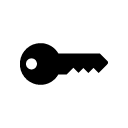
\includegraphics[scale=0.3]{img/key-128.png}};  
    \node (b) at (9.8,1) {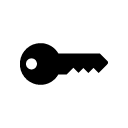
\includegraphics[scale=0.3]{img/key-128.png}};  
    \node (c) at (6,-1) {
\includegraphics[scale=0.05]{img/lock-128.png}};  
  \end{tikzpicture}
  \caption{The general strategy of a symmetric cryptography protocol.}
  \label{fig:crypto-sym}
\end{figure}
One famous example of an old cryptography protocol is the Caesar cipher, in
which each letter of the message is replaced by another letter. All the letters
are shifted by a constant number $n$ of positions down the alphabet. For
example, with $n=3$, the letter \texttt{D} becomes \texttt{A}, the letter
\texttt{E} becomes \texttt{B}, the letter \texttt{F} becomes \texttt{C}, and so
on. This encryption protocol is named after Julius Caesar,
who was using it to communicate with his family with the shift $n=3$. In
Figure~\ref{fig:caesar}, we draw the correspondence between the letters using
the shift $n=3$. The outer ring represent the letters in the \emph{plaintext}
(the original text, without encryption) while the inner ring represent the
letters in the \emph{ciphertext} (the text after the encryption).
\begin{figure}[h]
  \centering
  \begin{tikzpicture}[x=1em,y=1em]
%   set up
    \pgfmathsetmacro\angdiv{360/26}
    \pgfmathtruncatemacro\caeser{3} % Input Caeser shift here! (positive for clockwise)
    \coordinate (n-0) at (90+\angdiv/2:7) {};
    \coordinate (m-0) at (90-\caeser*\angdiv+\angdiv/2:5) {};
%   draw Caeser diagram
    \draw circle [radius=8] circle [radius=6.5] circle [radius=6]  circle [radius=4.5]
        \foreach \i in {0,...,25}{%
            ($({90-(\i-1/2)*\angdiv}:8)$) -- ($(({90-(\i-1/2)*\angdiv}:6.5)$)
            ($({90-(\i-1/2)*\angdiv}:4.5)$) -- ($(({90-(\i-1/2)*\angdiv}:6)$)
        };
    \foreach [count=\a from 0] \text in {A,B,...,Z}{
        \pgfmathtruncatemacro\b{\a+1}%
        \path [curved text=\text] (n-\a) arc [start angle=90-(\a-1/2)*\angdiv, delta angle=-\angdiv, radius=7] node (n-\b) {};
        \path [curved text=\text] (m-\a) arc [start angle=90-(\a+\caeser-1/2)*\angdiv, delta angle=-\angdiv, radius=5] node (m-\b) {}; % Inner circle
    }
%   draw arrow
    \draw [-latex, thick] (65:9.5) to[bend left=20,edge label=$+3$] (40:9.5);
    \end{tikzpicture}
  \caption{Representation of the Caesar cipher with a shift $n=3$.}
  \label{fig:caesar}
\end{figure}
In this example, the secret key of the protocol is the shift parameter $n$: if
you know $n$, you know both how to encrypt a message and how to decrypt one.
The Caesar cipher is simple enough to be executed by a machine, but it is not
used nowadays. Indeed, the number of keys one can choose when using the Caesar
cipher is rather small, so an adversary (a spy, an enemy...) can easily guess
what the message is after spending enough time trying all the possibilities. One could
even ask a computer to search for all the possible keys, thus recovering it even
faster. That is why, in modern cryptography, the number of possible keys must be
way bigger than this. For example, the standard protocol for symmetric
encryption, called AES (for Advanced Encryption Standard), was designed in
1999~\cite{DR99, DR02} and can be used with $2^{128}, 2^{192}$ or $2^{256}$
different possible keys, depending on the version used. The smallest of these
number can also be written as
\[
  2^{128} = 340282366920938463463374607431768211456,
\]
when a billion looks like
\[
  10^{9} = 1000000000,
\]
so they are really big numbers.

The number of possible keys is not the only thing that changed since Julius
Caesar. First, communication is now essentially digital, thus cryptography is
now a part of computer science. This is very important because it means that the
work in this thesis is also oriented towards computer science: we want to obtain
mathematical results that are effective, \ie usable by a computer.
Second, the scope of cryptography is now larger.
In modern cryptography, symmetric encryption is only one field of
cryptography, and there are many more aspects, such as asymmetric
encryption (also called \emph{public-key} encryption), data integrity,
authentication, digital signatures (the list is not exhaustive). We will not
explain all these terms, but the interested reader can look at the introductions
on each of these subjects in~\cite{MVOV18}, for example. An important change in
cryptography occured in 1976 with the seminal article \emph{New Directions in
Cryptography}~\cite{DH76} by Diffie and Hellman, with the invention of so called
public key cryptography. We briefly present public key encryption, in order to
compare it to symmetric encryption.

One of the main drawbacks of symmetric encryption is that the two
protagonists must have a secret in common in order to be able to securely
communicate. They can meet in person and agree on a secret, but this is not
always possible, for example if they live very far away of each other. They
could also find another way of communication, but then they cannot encrypt their
communication, because they do not share a secret yet and they want to
communicate precisely in order to share one. Thus, the problem of sharing a
secret seems to be unsolvable. In fact, public key encryption is an answer to
this problem, because it allows us to encrypt messages without the need for a
common secret. The elegant idea of Diffie and Hellman is to break the symmetry
between the participants (we will call them Alice and Bob, since it is
traditional to do so in cryptography). Instead of agreeing on a common key, only
one participant (for example Alice) creates a \emph{pair} of keys: one of them
is public and can be transmitted to anyone, while the other is private and must
be known by Alice only. With the public key, one can encrypt a message, while
the private key is necessary in order to decrypt an encrypted message. Using
such a system, everyone is able to send encrypted messages to Alice, because the
key used to do so is public, but only Alice can decrypt them. Thus, the
communications are secure.
\begin{figure}[h]
  \centering
  \begin{tikzpicture}
    \node (msg) at (0,0) {Message};
    \node (msg-enc) at (6,0) {Encrypted message};
    \node (msg-dec) at (12,0) {Decrypted message};
    \node (bob) at (0,2) {Bob};
    \node (alice) at (12, 2) {Alice};
    \node (key-pub) at (5, 2) {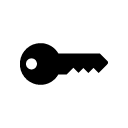
\includegraphics[scale=0.3]{img/key-128.png}};
    \node (key-pub-txt) at (5, 3) {Public key};
    \node (key-pri) at (7, 2) {
\includegraphics[scale=0.065]{img/key-512.png}};
    \node (key-pri-txt) at (7, 3) {Private key};
    \node (lock) at (6,-1) {
\includegraphics[scale=0.05]{img/lock-128.png}};  
    \draw[->] (msg) -- (msg-enc);
    \draw[->] (msg-enc) -- (msg-dec);
    \draw[->] (bob) to[bend left, edge label=Encrypts] (2.5,0);
    \node (key-pub2) at (2.2, .8) {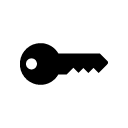
\includegraphics[scale=0.3]{img/key-128.png}};
    \draw[->] (alice) to[bend right, edge label = Decrypts] (9,0);
    \node (key-pri2) at (9.4, .8) {
\includegraphics[scale=0.065]{img/key-512.png}};
    \draw[->] (alice) to (8,2);
    \node (c) at (9.5, 2.3) {Creates};
  \end{tikzpicture}
  \caption{General concept of public-key encryption.}
  \label{fig:crypto-asym}
\end{figure}
We draw a diagram of the general idea in Figure~\ref{fig:crypto-asym}. With such
a system, Bob can only send messages to Alice. If Alice wants to send a message
to Bob using public-key cryptography, then Bob has to create his own pair of
keys. He then gives his public key to Alice, who can then encrypt her message
using this key and send it to Bob. Bob decrypts the message using his private
key. Public-key cryptography is somewhat heavier than symmetric
cryptography, hence another solution for Bob is to encrypt a secret and send it
to Alice, in order to be able to use symmetric encryption with that secret. This
is what is done in practice: only a \emph{key exchange} is performed using
public-key cryptography, the rest being handled by symmetric cryptography.
Still, public-key cryptography is fundamental, since it allows us to use
symmetric cryptography.

The first key exchange protocol was invented by Diffie and Hellman in
1976~\cite{DH76}, and an example of public-key encryption is given by the RSA
(named after Rivest, Shamir, and Adleman) protocol~\cite{RSA78} that was
described in 1977. These two protocols are both based on algebraic
structures. Indeed, mathematics are a handy way of studying and explaining
cryptography, for example the Caesar cipher with $n=3$ can be explained by
representing all letters by the numbers between $0$ and $25$
\[
  \texttt{A}\to 0, \texttt{B} \to 1, \dots,\texttt{Y}\to24, \texttt{Z}\to25
\]
and by defining the encryption as the subtraction by $3$. With this
representation, we have to agree that the number $-1$ is equivalent to the
number $25$, \ie before \texttt{A} comes \texttt{Z}, that $-2$ is equivalent to
$24$, \ie two times before \texttt{A} comes \texttt{Y}, and so on. In fact a
subpart of mathematics called \emph{number theory} is dedicated to the study of
this kind of numbers, together with some rules like the one that we just stated:
$-1=25$. These sets of numbers are called \emph{cyclic groups}, because they can
be represented on a circle, the one we spoke about is denoted by
\[
  \mathbb{Z}/26\mathbb{Z}
\]
and is represented in Figure~\ref{fig:cyclic-group}.
\begin{figure}[h]
  \centering
  \begin{tikzpicture}
    \foreach \x in {0, 1,...,25} \coordinate (\x) at (13.85*\x:3);
    \draw[additive-structure] (0,0) circle (3);
    \foreach \x in {0, 1,...,25} \draw[fill] (13.85*\x:3) circle (.1);
    \foreach \x in {0, 1,...,25} \node (p) at (13.85*\x:3.4) {$\x$};
  \end{tikzpicture}
  \caption{The cyclic group $\mathbb{Z}/26\mathbb{Z}$ represented on a circle.}
  \label{fig:cyclic-group}
\end{figure}
Many other interesting structures exist, see for example~\cite{Lang04, Perrin96}
for a course in algebra. With the growth of public-key cryptography, number
theory became its corner stone, and more advanced mathematical concepts were
used, like finite fields, elliptic curves or isogenies. Without entering into
the details of what these objects are, what is important is that the security of
cryptographic protocols relies on hard mathematical problems involving these
concepts. Thus, a better understanding of them means a better understanding of
the security of our cryptographic protocols. The part of cryptography that is
dedicated to the study of the security of cryptographic protocols (\ie how to
``break'' them) is called \emph{cryptanalysis}.

At the same time, since the protocols are based on the manipulation of these
objects, a better understanding of them also means better (in particular,
faster) cryptographic protocols. Since cryptography is everywhere in modern
communications (on the Internet, when you use your credit card, on messaging
applications on your smartphone, ...), efficient protocols are crucial. It is
thus necessary to be able to efficiently manipulate the mathematical concepts
behind our protocols both for cryptography (making efficient protocols) and
cryptanalysis (being able to analyze their security). By ``manipulate'', we mean
being able to do additions, multiplications, and sometimes more complicated
operations with these objects: the science studying how to do so is called
\emph{arithmetic}. In conclusion, it is necessary to have efficient arithmetic
for cryptography and cryptanalysis.

Examples of cryptographic protocols relying on finite field extension include
the quasi-polynomial algorithm for discrete logarithm in small characteristic by
Granger, Kleinjung and Zumbrägel~\cite{GKZ14}, where a tower of finite field
extensions is used. In the domain of curve-based cryptography, pairing friendly
curves~\cite{Joux00, FST10} are also defined on some finite field extension
$\mathbb{F}_{q^k}$.

\subsection*{Coding theory}
\addcontentsline{toc}{subsection}{Théorie des codes}
\label{sec:coding}

Another very elegant (and useful) application of finite fields is
\emph{coding theory}. Like cryptography, it is linked with communication,
although it adresses a different issue entirely. We now assume that Alice and
Bob want to communicate, and that the information they send go through a
channel. In practice, this channel could be optical fiber, electrical wires, radio
waves, and many more things. Assume that Alice wants to send the message ``Hi!
How are you?'' to Bob. In fact these letters would probably first be translated
into some stream of bits \texttt{0} and \texttt{1}, thus we will imagine that
Alice sends the message
\[
  m = \texttt{0010110001010111}
\]
through the cannel. Very often, in real conditions, the communication channel is
not perfect and is subject to \emph{channel noise}, \ie because of the quality of
the channel, or because of the environment, some errors can appear and change
the message sent by Alice into something else, as shown in
Figure~\ref{fig:communication-channel}.
\begin{figure}[h]
  \centering
  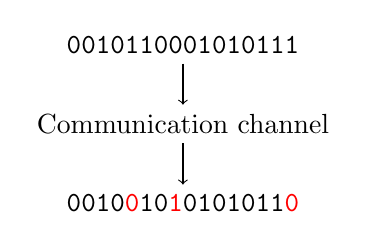
\begin{tikzpicture}
    \node (msg) at (0,2) {\texttt{0010110001010111}};
    \node (msg-dec) at (0,0)
    {\texttt{0010\textcolor{red}{0}10\textcolor{red}{1}0101011\textcolor{red}{0}}};
    \node (channel) at (0, 1) {Communication channel};
    \draw[->] (msg) -- (channel);
    \draw[->] (channel) -- (msg-dec);
  \end{tikzpicture}
  \caption{An imperfect communication channel.}
  \label{fig:communication-channel}
\end{figure}
Without any tool or context, it can be hard (or impossible) for Bob to guess
what was the initial message coming from Alice. Coding theory studies how to
make sure that Bob can recover the original message, even with some errors. The
goal is to build so-called \emph{codes} that can correct errors,
thus they are called \emph{error correcting codes} or \emph{error correction
codes}. The intuition is that in order to make sure that some
information, that is elementary reprensented by a \texttt{0} or a
\texttt{1}, arrives without error to Bob, Alice can just repeat it multiple
times. For example, if Alice repeats every bit three times, making words of
three symbols:
\[
  \texttt{0}\to\texttt{000}\quad\quad\texttt{1}\to\texttt{111},
\]
then an error can be corrected, because if Bob receives, for example, the
word \texttt{001}, he knows that is it most likely coming from
the word \texttt{000}, and he can interpret it as coming from the bit \texttt{0} in
Alice's initial message. More generally, if Bob receives the word
\texttt{abc}, he
interprets it as coming from the symbol \texttt{0} if there is a majority of
\texttt{0} in the word \texttt{abc}. Conversely, if there is a majority of
\texttt{1} in the word \texttt{abc}, he interprets the word as the symbol
\texttt{1}. Of course, if there are too much errors on a single word, it is
still possible to misinterpret it. For example, if the word
\texttt{000} becomes \texttt{110} after going through the communication channel,
then Bob will decode it as $\texttt{111}\to\texttt{1}$. This strategy is known
as the binary repetition code of
length $3$ and is an example of an error correction code. The whole procedure is
described in Figure~\ref{fig:rep3}.
\begin{figure}[h]
  \centering
  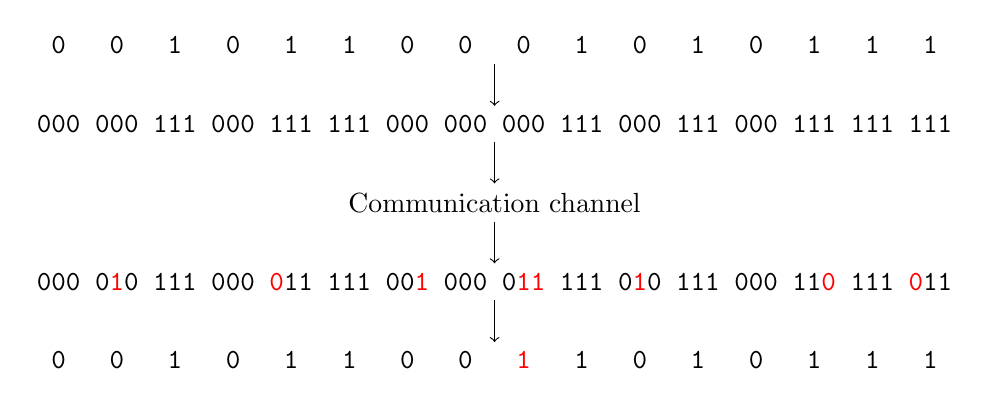
\begin{tikzpicture}
    \node (msg-init) at (0,3)
    {\texttt{\phantom{ }0\phantom{ } \phantom{ }0\phantom{ } \phantom{
    }1\phantom{ }  \phantom{ }0\phantom{ }  \phantom{ }1\phantom{ }  \phantom{
    }1\phantom{ }  \phantom{ }0\phantom{ }  \phantom{ }0\phantom{ }  \phantom{
    }0\phantom{ }  \phantom{ }1\phantom{ }  \phantom{ }0\phantom{ }  \phantom{
    }1\phantom{ }  \phantom{ }0\phantom{ }  \phantom{ }1\phantom{ }  \phantom{
    }1\phantom{ }  \phantom{ }1\phantom{ }}};
    \node (msg) at (0,2)
    {\texttt{000 000 111 000 111 111 000 000 000 111 000 111 000 111 111 111}};
    \node (msg-dec) at (0,0)
  {\texttt{000 0\textcolor{red}{1}0 111 000 \textcolor{red}{0}11 111
  00\textcolor{red}{1} 000 0\textcolor{red}{11} 111 0\textcolor{red}{1}0 111 000 11\textcolor{red}{0} 111 \textcolor{red}{0}11}};
    \node (channel) at (0, 1) {Communication channel};
    \node (msg-end) at (0,-1)
    {\texttt{\phantom{ }0\phantom{ } \phantom{ }0\phantom{ } \phantom{
    }1\phantom{ }  \phantom{ }0\phantom{ }  \phantom{ }1\phantom{ }  \phantom{
    }1\phantom{ }  \phantom{ }0\phantom{ }  \phantom{ }0\phantom{ }  \phantom{
    }\textcolor{red}{1}\phantom{ }  \phantom{ }1\phantom{ }  \phantom{ }0\phantom{ }  \phantom{
    }1\phantom{ }  \phantom{ }0\phantom{ }  \phantom{ }1\phantom{ }  \phantom{
    }1\phantom{ }  \phantom{ }1\phantom{ }}};
    \draw[->] (msg-init) -- (msg);
    \draw[->] (msg) -- (channel);
    \draw[->] (channel) -- (msg-dec);
    \draw[->] (msg-dec) -- (msg-end);
  \end{tikzpicture}
  \caption{The binary repetition code of length $3$.}
  \label{fig:rep3}
\end{figure}
In order to correct more errors, we could use repetition codes with bigger
lengths. Though, when we use a repetition code of length $n$, we have to send
$n$ times more information in the communication channel, which comes at a cost
in real life situations. We thus have to balance the cost coming from the length
of the code with the number of errors we want to be able to correct. In fact,
depending on the quality of the communication channel, all codes are not
suitable. Claude Shannon proved in
1948~\cite{Shannon48} that we can define a quantity called the \emph{capacity}
of the channel that essentially measures how much information we can send
through a communication channel. It also measures how much repetition we
must add in our code in order to send something through the communication
channel in a reliable way. Coding theory is still an active research field, thus
there are plenty of open problems and the question ``What is the best code we
can use?'' has no definitive answer. The codes used in practice
are a bit more subtle that the repetition code, even if they follow the same
logic. Finite fields are used to represent and manipulate codewords of error
correction codes. For example, the Reed-Solomon codes~\cite{RS60}, that are used
in consumer technologies like CDs, DVDs, Blu-ray discs, QR codes, but also in
space NASA missions, use sequences of values taken in a finite field as
codewords. Some other codes, like the geometric Goppa codes~\cite{Goppa81}, are
based on algebraic function fields, a mathematical structure that is based on
top of finite fields and involves finite field extensions.
In conclusion, exactly like in cryptography, finite fields are
ubiquitous in coding theory, and efficient arithmetic in finite fields ensures
at the same time fast coding and fast decoding.

\section*{Finite fields arithmetic}
\addcontentsline{toc}{section}{Arithmétique des corps finis}

As stated in Sections~\ref{sec:crypto} and~\ref{sec:coding}, cryptographic
protocols and codes rely on
mathematical structures in order to work. The one we will study throughout this
document is called \emph{finite field}. A \emph{field} is a mathematical
structure (we also say \emph{algebraic structure}) composed of elements that we
can \emph{add}, \emph{substract}, \emph{multiply}, and \emph{divide} (except by
zero). It is a well-known algebraic structure: for example the set of real
numbers, denoted by $\mathbb{R}$, is a field. Indeed, the elements in
$\mathbb{R}$, for example $0, 1, -3, 5631$ but also more complicated numbers
such as $\pi, \sqrt 2, \frac{7}{13}$ can be added, substracted, multiplied or
divided. Numbers in $\mathbb{R}$ can have an infinite number of decimals, for
example the $60$ first decimals of the constant $\pi$ are
\[
  \pi = 3.14159265358979323846264338327950288419716939937510582097494\dots.
\]
A computer only has a finite memory, \ie the quantity of information it can
store is finite. As a consequence, it is impossible to store all the decimals of
$\pi$, and, more generally, the decimals of a lot of numbers in $\mathbb{R}$. It
is still possible to work with numbers in $\mathbb{R}$ on a computer, but it is
somewhat harder than to work with elements in a \emph{finite} algebraic
structure, \ie a set composed of $n$ elements, with
\[
  n < \infty.
\]
One example of such a structure was given in Section~\ref{sec:crypto}: the
cyclic groupe $\mathbb{Z}/26\mathbb{Z}$ that is composed of the ``numbers'' $0,
1, \dots, 25$. They are not the same numbers as those we know though, since with
the elements of $\mathbb{Z}/26\mathbb{Z}$ we have, for example
\[
  3 - 4 = -1 = 25,
\]
and this is not true for the actual numbers in $\mathbb{R}$, but we still write
them the same way for convenience. We already defined an
addition and substraction on $\mathbb{Z}/26\mathbb{Z}$, and we could also define
a multiplication and a division in a very natural way. Finite fields are a
generalization of spaces like
$\mathbb{Z}/26\mathbb{Z}$. The set $\mathbb{Z}/26\mathbb{Z}$ is not a field for
technical reasons, but to think of finite fields as sets like this is a good
enough approximation for this introduction.

Because the elements of a finite field are, by definition, finite, they are
somewhat easier to manipulate on a computer. Moreover, the field structure
allows us to manipulate the elements like usual numbers (\ie with additions,
multiplications, ...), which makes them useful. This is why today, finite fields
are everywhere in cryptography, but also in other domains at the crossroad of
mathematics and computer science, like coding theory.

Sometimes, simple mathematical problems are well understood on a theoretical
point of view, but there are still open questions concerning practical aspects.
For example, the multiplication of two integers $a$ and $b$ in $\mathbb{N}$ is a
simple problem, that can be done by hand by children. Still, the question of how
to compute it on a computer (in an optimal way) is open, and there are still
research articles~\cite{HVDH19} on that problem.
Finite field arithmetic (\ie how to perform operations such as additions and
multiplications) is very well understood, because the finite field structure is
rather simple. But again, the best way of multiplying two elements in a finite
field is still unknown. This is the subject of this thesis: the study of the
finite field arithmetic.

\section*{Résumé des travaux}
\addcontentsline{toc}{section}{Résumé des travaux}

Ce résumé présente de manière détaillée l'ensemble des travaux réalisés pendant
ma thèse, ainsi que la façon dont est organisé ce manuscrit. Cette partie est
donc dédiée à un ``public scientifique averti''.

\subsection*{Arithmétique efficace dans une extension fixée}
\addcontentsline{toc}{subsection}{Arithmétique efficace dans une extension fixée}

Ce document est composé de deux parties, qui sont essentiellement indépendantes.
Dans la Partie~\ref{part:single}, nous étudions l'arithmétique d'une extension
de corps fini fixée
\[
  \mathbb{F}_{p^{k}}.
\]
\paragraph{Préliminaires.} Nous commençons dans le
Chapitre~\ref{chap:preliminary} par rappeler les faits fondamentaux concernant
les objets que nous utiliserons dans le reste du document. En particulier, on
rappelle la structure des corps finis, ainsi que la manière de les construire
comme des quotients d'anneaux de polynômes
\[
  \mathbb{F}_p[x]/(P(x)).
\]
Nous donnons quelques propriétés des extensions de corps finis concernant leur
structure d'espace vectoriel ainsi que sur leur groupe d'automorphismes.

Dans la Section~\ref{sec:algebraic-function-fields}, nous présentons les
\emph{corps de
fonctions algébrique}, une structure algébrique que nous utilisons dans les
preuves des Chapitres~\ref{chap:bilinear} et~\ref{chap:hypersymmetric}. On
rappelle brièvement ce que sont les \emph{places}, et qu'elles sont
essentiellement équivalentes aux notions de valuations discrètes et d'anneaux de
valuations. On décrit comment évaluer un élément $z$ d'un corps de fonction
algébrique à une place $P$, et on donne la définition d'un zéro et d'un pôle, ce
qui justifie le nom de corps de ``fonction''. Enfin, on donne la définition d'un
\emph{diviseur} et on rappelle les résultats habituels de la théorie : le lien
entre le degré et la dimension d'un diviseur, la définition du \emph{genre} d'un
corps de fonctions algébrique, et le théorème de Riemann-Roch.

Dans la Section~\ref{sec:complexity-models}, on donne le modèle de la
\emph{complexité algébrique} et on explique pourquoi ce modèle est pertinent
pour nos travaux. On rappelle également les notions de \emph{grand O} et
\emph{petit o}, qui sont utilisées pour exprimer des résultats asymptotiques.

Enfin, dans la Section~\ref{sec:fundamental-algos}, nous donnons des références
bibliographiques, ainsi que la complexité de certains algorithmes classiques et
important dans notre travail : l'algorithme de Brent-Kung pour la composition
modulaire, le calcul de polynôme minimal, et l'algorithme de Berlekamp-Massey.
Ces routines sont utilisés dans plusieurs algorithmes de ce manuscrit, notamment
dans les Chapitres~\ref{chap:isomorphism} et~\ref{chap:standard}.

\paragraph{Complexité bilinéaire et algorithmes de type Chudnovsky$^2$.} Dans le
Chapitre~\ref{chap:bilinear}, nous présentons la théorie de la \emph{complexité
bilinéaire}, un modèle alternatif de complexité utilisé pour mesurer le coût de
calcul de certaines applications bilinéaires. Dans ce modèle, seules les
multiplications sont comptées, ce qui est justifié par le fait qu'en pratique
les multiplications sont plus coûteuse que les additions. La complexité
bilinéaire d'une application est alors donnée par le nombre minimal de
multiplications nécessaires au calcul de l'application en question. L'algorithme
de Karatsuba est un exemple pratique de l'intérêt de ce modèle de complexité. En
effet, l'idée derrière cet algorithme est de multiplier deux polynômes de degré
$1$
\[
  A = a_1 X + a_0\text{ et }B = b_1 X + b_0
\]
avec seulement trois produits
\[
  c_0 = a_0b_0,
\]
\[
  c_1 = (a_0+a_1)(b_0+b_1),
\]
et
\[
  c_\infty = a_1b_1,
\]
à la place des quatre produits classiques $a_0b_0$, $a_0b_1$, $a_1b_0$ et
$a_1b_1$ comme suit :
\[
  AB = c_\infty X^2 + (c_1-c_\infty-c_0) X + c_0.
\]
Dans la Section~\ref{sec:bilinear-complexity}, après avoir rigoureusement
définit la complexité bilinéaire d'une application bilinéaire $\Phi$ en
utilisant des \emph{formules bilinéaires}, nous expliquons que cette définition
est en réalité équivalente au rang du tenseur correspondant à $\Phi$. Nous
présentons également la version \emph{symétriques} de la complexité bilinéaire,
qui compte le nombre minimal de multiplications symétriques nécessaire au calcul
de $\Phi$, et qui est également étudiée dans la littérature. Nous sommes
particulièrement intéressés par la multiplication dans les extensions de corps
finis, et par sa complexité bilinéaire (symétrique).

Dans la Section~\ref{sec:chudchud-algo}, nous redonnons le principe
d'évaluation-interpolation et nous présentons un algorithme dû à Chudnovsky et
Chudnovsky~\cite{CC88} basé sur l'évaluation et l'interpolation sur des places
de corps de fonctions algébrique. Cet algorithme fondateur donne une borne
asymptotique \emph{linéaire} en le degré de l'extension, que ce soit pour la
complexité bilinéaire ou la complexité bilinéaire symétrique de la
multiplication dans une extension de corps fini. Il a été très étudié, et nous
présentons brièvement quelques améliorations~\cite{BR04, CO10, Randriam12}.

Toutefois, l'algorithme de Chudnovsky et Chudnovsky donne uniquement une borne
sur la complexité bilinéaire, qui s'avère être asymptotiquement bonne. Ainsi,
nous donnons aussi dans la Section~\ref{sec:algorithmic-searches} un algorithme
de Barbulescu, Detrey, Estibal et Zimmermann~\cite{BDEZ12} qui permet de
calculer la complexité bilinéaire en petite dimension. Leur algorithme énumère
toutes les formules biinéaires pour une longueur donnée, et peut ainsi être
utilisé pour obtenir la longueur minimale d'une formule permettant de calculer
une application bilinéaire $\Phi$, autrement dit cet algorithme permet de
calculer la complexité bilinéaire de $\Phi$. L'algorithme est expliqué en
détails, et quelques améliorations dûes à Covanov~\cite{Covanov19} sont
mentionnées.

\paragraph{Complexité bilinéaire hypersymétrique.} Dans le
Chapitre~\ref{chap:hypersymmetric}, nous nous intéressons à de nouveaux modèles
de complexité, et nous donnons des résultats à la fois en petite dimension et
asymptotiquement. Dans la Section~\ref{sec:sym-and-hypersym}, nous généralisons
la notion de complexité bilinéaire dans le cas du produit de $s\geq2$ variables
\[
  x_1\times x_2 \times\dots x_{s-1}\times x_s
\]
dans une extension de corps fini $\mathbb{F}_{p^{k}}$. En adaptant l'algorithme
de Chudnovsky et Chudnovsky dans ce cas, nous montrons dans la
Section~\ref{sec:asymptotic} que cette \emph{complexité multilinéaire} reste
linéaire en le degré $k$ de l'extension, comme dans le cas de la complexité
bilinéaire classique.

Dans ce chapitre, on définit également une nouvelle complexité appelée
\emph{complexité bilinéaire hypersymétrique}, qui est inspiré de la complexité
bilinéaire symétrique usuelle, dans laquelle une condition de symétrie
additionnelle est étudiée. Dans la Section~\ref{sec:algo-small-dim}, nous
donnons un alorithme \emph{ad hoc} de recherche
de formules hypersymétriques, inspiré par l'algorithme de Barbulescu, Detrey,
Estibal and Zimmermann, qui nous permet de calculer la complexité bilinéaire
hypersymétrique. Nous analysons notre algorithme en détails, et donnons des
résultats expérimentaux issus de notre implémentation, dans le cas de la
multiplication dans les extensions de corps finis. En utilisant des
\emph{formules universelles}, c'est-à-dire des formules qui sont vraies pour
presque tout nombre premier $p$, nous donnons aussi des résultats théoriques
concernant la complexité bilinéaire hypersymétrique dans les extensions de corps
finis
\[
  \mathbb{F}_{p^{k}}
\]
et dans des algèbres de polynômes tronqués
\[
  \mathbb{F}_p[T]/(T^k)
\]
en petite dimension $k$, qui généralisent des résultats connus pour la
complexité bilinéaire. Nous obtenons également la linéarité de la complexité
bilinéaire hypersymétrique de la multiplication dans l'extension
$\mathbb{F}_{p^{k}}$ en le degré de l'extension $k$, comme corollaire du même
résultat pour la complexité multilinéaire.

\subsection*{Arithmétique efficace dans un réseau d'extensions}
\addcontentsline{toc}{subsection}{Arithmétique efficace dans réseau d'extensions}

Dans la Partie~\ref{part:lattice}, nous étudions comment gérer plusieurs
corps finis simultanément, dans ce que l'on appelle un \emph{réseau de corps
finis compatiblement plongés}. D'un point de vue théorique, cela revient à se
demander comment calculer dans la clôture algébrique
\[
  \bar{\mathbb{F}}_{p} = \bigcup_{k\geq1}\mathbb{F}_{p^k}
\]
du corps de base $\mathbb{F}_p$.

\paragraph{Algorithmes d'isomorphisme.} Le Chapitre~\ref{chap:isomorphism} est
dédié au problème de l'isomorphisme, qui demande de calculer efficacement un
isomorphisme (ou plus généralement un plongement)
\[
  K\emb L
\]
entre deux corps finis $K$ et $L$. Dans la Section~\ref{sec:prelim-naive-algo},
nous exposons le problème de l'isomorphisme, et, suivant la présentation faite
dans~\cite{BDDFS17}, nous le divisons en deux parties : le problème de la
description du plongement et le problème de l'évaluation du plongement. Le
problème de la description du plongement consiste à trouver des éléments
$\alpha\in K$ et $\beta\in L$ tels que
\[
  K = \mathbb{F}_{p}(\alpha)
\]
et tel qu'il existe un plongement $\phi:K\emb L$ qui envoie $\alpha$ vers
$\beta$. Connaissant $\alpha$ et $\beta$, le problème de l'évaluation du
plongement consiste alors à évaluer $\phi$ de manière efficace. Nous traitons
d'abord le problème de la description et nous présentons l'algorithme naïf, basé
sur la factorisation de polynômes, dans la
Section~\ref{sec:embedding-description}.

Dans la Section~\ref{sec:allombert}, nous présentons un algorithme plus élaboré
dû à Allombert~\cite{Allombert02} et inspiré par le travail de
Lenstra~\cite{Lenstra91}, que nous appelons algorithme de Lenstra-Allombert.
L'algorithme de Lenstra-Allombert est basé sur la théorie de Kummer, qui étudie
certaines extensions de corps, et utilise des racines primitives de l'unité. Si
l'extension $\mathbb{F}_{p^{n}}$ admet une racine $n$-ième de l'unité primitive
$\zeta_n$,
alors la description de l'algorithme est plus simple et est donnée dans la
Section~\ref{sec:preliminaries}. Sinon, il est nécessaire d'ajouter
artificiellement une racine $\zeta_n$ à l'extension $\mathbb{F}_{p^{n}}$, ce qui
nous conduit à étudier les algèbres de la forme
\[
  A_n = \mathbb{F}_{p^{n}}\otimes\mathbb{F}_p(\zeta_n)
\]
que nous appelons \emph{algèbres de Kummer}. Les éléments $\alpha$ et $\beta$
décrivant le plongement donnés par l'algorithme de Lenstra-Allombert sont alors
déduits des solutions d'équations de la forme
\[
  (\sigma\otimes1)(x) = (1\otimes\zeta)x
\]
dans des algèbres de Kummer. Ces équations sont appelées Hilbert $90$. Les
algèbres de Kummer, ainsi que les solutions de Hilbert $90$, sont étudiées en
détail dans la Section~\ref{sec:kummer-algebras}, car elles jouent un rôle
central dans le Chapitre~\ref{chap:standard}.

En utilisant les résultats de la Section~\ref{sec:kummer-algebras}, nous
expliquons dans la Section~\ref{sec:lenstra-allombert-isomorphism} comment
obtenir les éléments $\alpha$ et $\beta$ des solutions de Hilbert $90$. Puis,
on présente les techniques pour obtenir les solutions de Hilbert $90$ dans la
Section~\ref{sec:computing-h90}. Enfin, les techniques standards permettant de
répondre au problème de l'évaluation du plongement sont traitées dans la
Section~\ref{sec:evaluation}.
%
